{\bf Introduction}

\begin{center}
    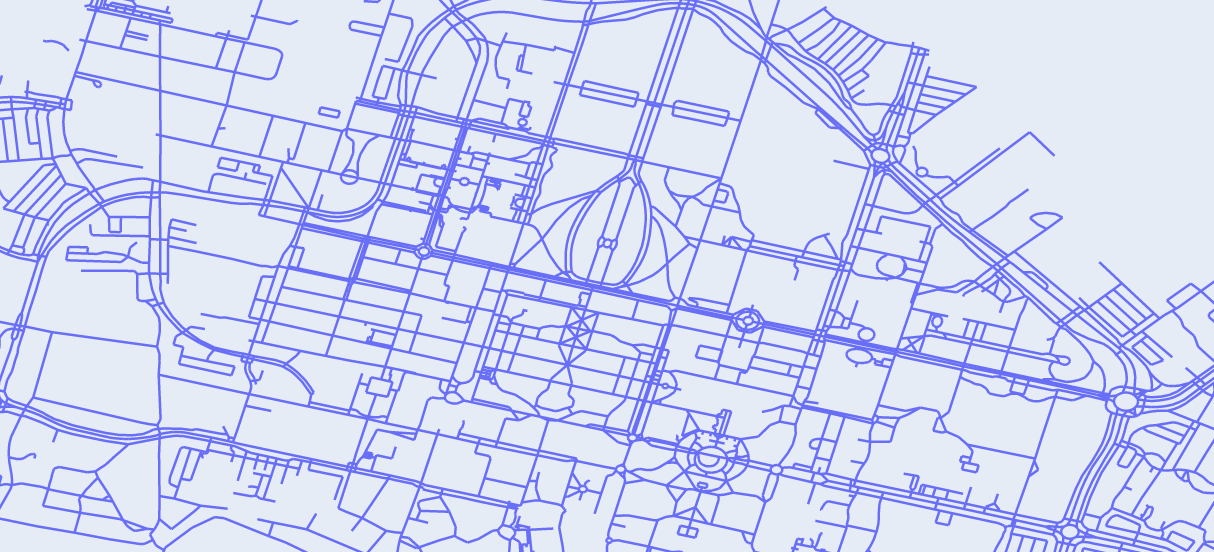
\includegraphics[width=1\textwidth]{stanford-map.png}
\end{center}

In route planning, the objective is to find the best way to get from point A to point B (think Google Maps). In this homework, we will build on top of the classic shortest path problem to allow for more powerful queries. For example, not only will you be able to explicitly ask for the shortest path from the Gates Building to Coupa Cafe at Green Library, but you can ask for the shortest path from Gates back to your dorm, stopping by the package center, gym, and the dining hall (in any order!) along the way.

We will assume that we have a \textit{map} of a city (e.g., Stanford) consisting of a set of \textit{locations}. Each location has:

\begin{enumerate}
    \item a unique label (e.g., 6608996258),
    \item a (latitude, longitude) pair specifying where the location is (e.g., 37.4299866, -122.175519), and
    \item a set of \textit{tags} which describes the type of location (e.g., amenity=food).
\end{enumerate}

There are a set of \textit{connections} between pairs of locations; each connection has a \textit{distance} (in meters), and can be traversed in both directions (if the distance from A to B is 100 meters, then the distance from B to A is also 100 meters).

There are two city maps that you'll be working with: a grid map (|createGridMap|) and a map of Stanford (|createStanfordMap|), which is derived from \href{https://www.openstreetmap.org/}{Open Street Maps}. We have also included instructions on how to create your own maps in |README.md|.
